\documentclass[tikz,border=6pt]{standalone}
\usepackage{tikz}
\usetikzlibrary{arrows.meta,positioning}
\definecolor{ink}{HTML}{222222}
\definecolor{stagefill}{HTML}{E8F1FF}
\definecolor{gatefill}{HTML}{FFF4D6}
\tikzset{
  stage/.style={draw=ink, rounded corners=2pt, very thick, align=center, minimum height=11mm, text width=27mm, fill=stagefill, font=\sffamily\small},
  gate/.style={draw=ink, rounded corners=2pt, thick, align=center, text width=30mm, fill=gatefill, font=\sffamily\footnotesize},
  arrow/.style={-{Latex[length=2.2mm]}, very thick, draw=ink}
}
\begin{document}
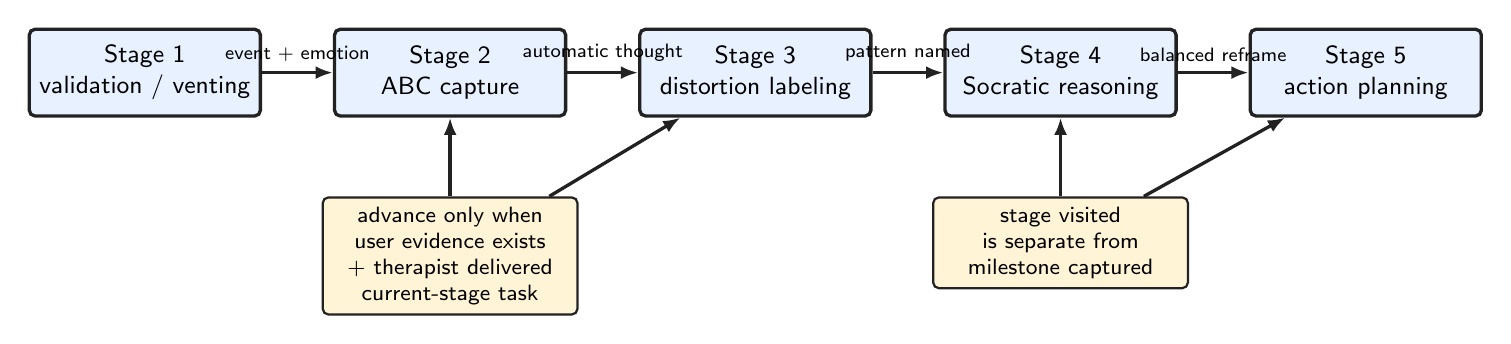
\begin{tikzpicture}[node distance=9mm]
  \node[stage] (s1) {Stage 1\\validation / venting};
  \node[stage, right=of s1] (s2) {Stage 2\\ABC capture};
  \node[stage, right=of s2] (s3) {Stage 3\\distortion labeling};
  \node[stage, right=of s3] (s4) {Stage 4\\Socratic reasoning};
  \node[stage, right=of s4] (s5) {Stage 5\\action planning};

  \node[gate, below=10mm of s2] (g1) {advance only when\\user evidence exists\\+ therapist delivered\\current-stage task};
  \node[gate, below=10mm of s4] (g2) {stage visited\\is separate from\\milestone captured};

  \draw[arrow] (s1) -- node[above, font=\sffamily\scriptsize] {event + emotion} (s2);
  \draw[arrow] (s2) -- node[above, font=\sffamily\scriptsize] {automatic thought} (s3);
  \draw[arrow] (s3) -- node[above, font=\sffamily\scriptsize] {pattern named} (s4);
  \draw[arrow] (s4) -- node[above, font=\sffamily\scriptsize] {balanced reframe} (s5);
  \draw[arrow] (g1) -- (s2);
  \draw[arrow] (g1) -- (s3);
  \draw[arrow] (g2) -- (s4);
  \draw[arrow] (g2) -- (s5);
\end{tikzpicture}
\end{document}
